\documentclass[11pt,a4paper]{article}

% --- Packages ---------------------------------------------------------------
\usepackage[margin=1in]{geometry}
\usepackage[utf8]{inputenc}
\usepackage[T1]{fontenc}
\usepackage{lmodern}
\usepackage{amsmath,amssymb,amsthm}
\usepackage{graphicx}
\usepackage{booktabs}
\usepackage{multirow}
\usepackage{array}
\usepackage{caption}
\usepackage{subcaption}
\usepackage{siunitx}
\usepackage{microtype}
\usepackage{xcolor}
\usepackage[hidelinks]{hyperref}
\usepackage{cleveref}
\usepackage{listings}

\sisetup{group-separator={,}}

% Absorb minor line-end overflows from long \texttt{} tokens.
\emergencystretch=3em

\title{Ranking Critical Links in the Kanto
500/275~kV Power Grid}

\author{NetworkEntropy Research Project\\
\small{Code repository: \texttt{NetworkEntropy} (branch \texttt{iterative-method})}}

\date{April 2026}

% --- Document ---------------------------------------------------------------
\begin{document}
\maketitle

\begin{abstract}
We treat the Kanto high-voltage power grid as a network and rank its
transmission lines by how critical each one is to keeping the grid
connected. The network is the \SI{500}{\kilo\volt} and
\SI{275}{\kilo\volt} backbone run by TEPCO and J-Power across eastern
Japan. From the ComplexNetTSP power-grids dataset, which was extracted
from OpenStreetMap, we take the largest connected component
(\num{156} nodes, \num{190} edges) and rank its edges with nine metrics:
local degree (LDC), neighbourhood overlap (Jaccard), $k$-shell (LKS),
Collective Influence (four variants), Link-Local Betweenness Centrality
(LLBCe), and its mapping-entropy extension (LLBMEe1). We score each
metric by removing edges in rank order and measuring the area under the
relative-giant-component (RGC) curve; a lower area means the metric
finds critical edges sooner. In the static case, LLBCe gives the lowest
area ($0.174$), about \SI{21}{\percent} better than the next metric
(Jaccard, $0.220$). When ranks are recomputed after each removal (the
iterative case), the CI variants improve sharply, but LLBCe keeps the
lead by a smaller margin. We also identify the seven trunk hubs of the
\SI{500}{\kilo\volt} grid and describe the chain of bridges that links
the TEPCO service area to outlying regions.
\end{abstract}

\section{Introduction}
\label{sec:intro}

Power grids are a standard example of critical infrastructure whose
failure modes depend as much on network topology as on the
electromechanical properties of any single component. Past cascading
failures, such as the 2003 North American blackout and the 2018 Taiwan
brownout, showed that removing a small number of structurally exposed
transmission corridors in sequence can disconnect tens of millions of
customers~\cite{albert2004structural,buldyrev2010catastrophic}.

In Japan, the Kanto region around Tokyo (roughly longitude
$138.3^{\circ}$E to $141.0^{\circ}$E and latitude $34.8^{\circ}$N to
$37.1^{\circ}$N) has the highest electricity demand density in the
country. It is served entirely at \SI{50}{\hertz} by Tokyo Electric
Power Company (TEPCO) and Electric Power Development
(``J-Power'')~\cite{tepco2024network}. Conversion to the western
\SI{60}{\hertz} grid passes through only three back-to-back DC
substations with limited capacity, so the internal resilience of the
Kanto grid effectively sets the black-start capability for the eastern
half of the country.

This paper applies network dismantling to the Kanto
\SI{500}{\kilo\volt}/\SI{275}{\kilo\volt} backbone and asks one
question: \emph{which transmission edges, when removed, fragment the
bulk-power network fastest?} We compare nine edge-ranking metrics from
the recent link-criticality literature. We test each under a static
regime (rank once, then remove) and an iterative regime (rank, remove,
then recompute), and report what the results mean for vulnerability
assessment.

\section{Background and Related Work}
\label{sec:background}

\subsection{Edge ranking and network dismantling}
The dismantling problem~\cite{braunstein2016network} asks for the
smallest set of nodes (or edges) whose removal drops the largest
connected component below a target size. For the edge version, a ranking
heuristic is usually judged by the relative-giant-component (RGC) curve
as a function of the fraction of edges removed, summarised by the area
under the curve (AUC):
\begin{equation}
\text{AUC}(M) = \int_0^1 \text{RGC}\bigl(f \mid \text{order}_M\bigr)\, df
\label{eq:auc}
\end{equation}
where $\text{order}_M$ is the removal order induced by metric $M$. A
lower AUC means the metric puts critical edges earlier in the removal
sequence.

\subsection{Power-grid topology}
GridKit~\cite{wiegmans2016gridkit} extracted high-voltage transmission
networks from OpenStreetMap (OSM) for Europe and North America, but it
does \emph{not} cover Japan. The ComplexNetTSP/Power\_grids
project~\cite{complexnettsp2023} built an equivalent extraction for
Japan directly from raw OSM \texttt{power=*} tags. It gives two CSV
files: one for vertices (substations and line-segment junctions) and one
for edges (transmission lines). We use this source.

\subsection{Edge criticality metrics}
We test nine metrics from three families. \textbf{Topological:}
Link Degree Centrality (LDC, $k_u \cdot k_v$), the Jaccard index of
neighbourhood overlap, and Link $k$-Shell (LKS, $\text{core}(u) \cdot
\text{core}(v)$). \textbf{Influence-based:} four variants of edge-level
Collective Influence (CI) at radius $\ell{=}3$, which separate the ball
``skin'' (nodes at exactly distance $\ell$) from the ball ``body''
(nodes within distance $\ell$) and aggregate endpoint scores to edges by
either average or product~\cite{morone2015influence,kitsak2024edge}.
\textbf{Entropy-based:} Link-Local Betweenness Centrality (LLBCe) and
its mapping-entropy extension (LLBMEe1)~\cite{li2024llbce}. The last two
are recent and need care to implement; see \Cref{sec:methods}.

\section{Data and Network Construction}
\label{sec:data}

\subsection{Source data}
We start from \texttt{japan\_nodes.csv} and \texttt{japan\_edges.csv} in
the ComplexNetTSP Power\_grids release. Each vertex carries a
\texttt{v\_id}, longitude and latitude (WGS-84, EPSG:4326),
\texttt{voltage} (volts), \texttt{frequency}, a \texttt{name} (Japanese,
with romaji where present), an \texttt{operator}, and a \texttt{typ}
(substation, generator, joint, and so on). Each edge carries its two
endpoints.

\subsection{Geographic filter and largest connected component}
We restrict the data to a Kanto bounding box
\(\text{lon} \in [138.3, 141.0],\ \text{lat} \in [34.8, 37.1]\)
and take the largest connected component (LCC) of the resulting
subgraph. This gives:
\begin{itemize}
\item \num{156} nodes (\num{99} named substations or labelled junctions,
\num{57} unlabelled OSM line-segment vertices),
\item \num{190} edges,
\item \num{56} bridges and \num{54} articulation points,
\item diameter \num{23},
\item degree distribution
$[\,(1,29),(2,66),(3,39),(4,14),(5,3),(6,4),(7,1)\,]$
giving a mean degree $\bar k = \num{2.44}$.
\end{itemize}
All retained nodes run at \SI{50}{\hertz}. Despite the loose longitude
bound, no Chubu (\SI{60}{\hertz}) substation falls inside the box: the
east-west frequency boundary at the Fuji and Sakuma converter stations
sits just west of it.

\subsection{Verification}
We spot-checked \num{10}/\num{10} randomly chosen named substations and
confirmed real TEPCO/J-Power facilities at the listed coordinates:
Shin-Tokorozawa, Shin-Tama, Shin-Keiyo, Shin-Hadano, Shin-Okabe,
B\=os\=o, Shin-Haruna, Shin-Sawara, Katsunan, and Shin-Fuji. We checked
the top-degree hubs against TEPCO's published \SI{500}{\kilo\volt}
backbone illustration~\cite{tepco2024network}.

\subsection{Caveats}
Of the \num{156} LCC nodes, \num{57} are unlabelled OSM line-segment
junctions: points where a mapper split a transmission corridor into
several OSM ways for tagging or vertex-density reasons, not actual
substations. They inflate the apparent diameter and add to the \num{56}
bridges. We keep them because removing them changes edge counts and
would bias the comparison. A reader who wants the substation-only
topology can collapse them by merging degree-2 unnamed vertices.

\subsection{Regional decomposition}
A coarse split by lon/lat box (\Cref{tab:regions}) places the network's
centre in the Tokyo metropolitan area: \num{35}\,\% of edges fall in
Tokyo Metro West and East combined, and \num{18}\,\% are inter-region
corridors that form the most exposed bridges.

\begin{table}[h]
\centering
\small
\caption{Regional decomposition of the Kanto LCC by coarse lon/lat box.}
\label{tab:regions}
\begin{tabular}{lrrr}
\toprule
Region & Nodes & Named & Intra-edges \\
\midrule
NE Kanto (Ibaraki S / N Chiba) & 36 & 19 & 41 \\
Tokyo Metro West              & 35 & 26 & 36 \\
Tokyo Metro East / Chiba      & 26 & 16 & 20 \\
NW Kanto (Saitama / W Tokyo)  & 20 & 9 & 22 \\
South Kanto (Kanagawa / W Izu)& 17 & 14 & 17 \\
North Kanto (Gunma / Tochigi) & 14 & 9 & 13 \\
South Kanto (S Chiba / B\=os\=o)  & 8 & 6 & 6 \\
\midrule
Inter-region edges            & --- & --- & 35 \\
\bottomrule
\end{tabular}
\end{table}

\section{Methods}
\label{sec:methods}

\subsection{Notation and conventions}
Let $G = (V, E)$ with $|V| = N$ and $|E| = m$. Let $k_v = \deg_G(v)$ and
$N(v) = \{u : (u,v) \in E\}$. All metrics produce a Pandas DataFrame with
columns $\{i, j, M_1, \dots, M_q\}$, where $(i,j)$ is the edge and
$M_1, \dots, M_q$ are scalar scores.

\subsection{Topological metrics}
\begin{align}
\text{LDC}(u,v)     &= k_u \cdot k_v, \\
\text{Jaccard}(u,v) &= \frac{|N(u) \cap N(v)|}{|N(u) \cup N(v)|}, \\
\text{LKS}(u,v)     &= \text{core}(u) \cdot \text{core}(v),
\end{align}
where $\text{core}(\cdot)$ is the $k$-core index from peeling.

\subsection{Collective Influence (four variants)}
For radius $\ell = 3$, define the ball boundary
$\partial \text{Ball}(u, \ell) = \{w : d_G(u,w) = \ell\}$ and the ball
volume $\text{Ball}(u, \ell) = \{w : 0 < d_G(u,w) \le \ell\}$. The
node-level CI is then
\begin{equation}
\text{CI}_S(u) = (k_u - 1) \sum_{w \in \partial\text{Ball}(u, \ell)} (k_w - 1),
\quad
\text{CI}_B(u) = (k_u - 1) \sum_{w \in \text{Ball}(u, \ell)} (k_w - 1).
\end{equation}
We aggregate these to edges by arithmetic mean or product of the
endpoint scores, which gives four edge-level columns:
$\text{CI\_e\_av\_skin}, \text{CI\_e\_mul\_skin},
\text{CI\_e\_av\_body}, \text{CI\_e\_mul\_body}$.

\subsection{LLBCe and LLBMEe1}
For an edge $e = (u,v)$, define the first-order central domain
\begin{equation}
\Gamma(e) \;=\; \{u, v\} \,\cup\, N(u) \,\cup\, N(v).
\end{equation}
The Link-Local Betweenness Centrality is then
\begin{equation}
\text{LLBCe}(e) \;=\; \frac{1}{|\Gamma(e)|\bigl(|\Gamma(e)| - 1\bigr)}
\sum_{\substack{s,t \in \Gamma(e) \\ s \ne t}}
\frac{\sigma_{st}(e)}{\sigma_{st}},
\label{eq:llbce}
\end{equation}
where $\sigma_{st}$ is the number of shortest paths between $s$ and $t$
in $G$, and $\sigma_{st}(e)$ is the number of those paths that pass
through $e$. The source and target sets are restricted to $\Gamma(e)$,
but the path computation stays in the full graph $G$. We do not extract
a subgraph, because that would change shortest-path lengths and give
different rankings. We implement \Cref{eq:llbce} with NetworkX's
\texttt{edge\_betweenness\_centrality\_subset}, setting both
\texttt{sources} and \texttt{targets} to $\Gamma(e)$, then dividing the
unnormalised output by $|\Gamma(e)|(|\Gamma(e)|{-}1)$.

The mapping entropy LLBMEe1 measures how concentrated the LLBCe values
are across the edges that touch either endpoint of $e_1$:
\begin{equation}
\text{LLBMEe1}(e_1) = -\sum_{e_k \in \Gamma_E(e_1)}
p_k \log p_k,
\quad
p_k = \frac{\text{LLBCe}(e_k)}{\sum_{e_j \in \Gamma_E(e_1)} \text{LLBCe}(e_j)},
\label{eq:llbme}
\end{equation}
where $\Gamma_E(e_1)$ is the set of edges incident to $u$ or $v$. An
edge whose neighbourhood mass sits on one dominant neighbour gives a low
LLBMEe1; an edge in a uniform bottleneck gives a high one.

\subsection{Static and iterative dismantling}
Given a metric $M$, the \emph{static} curve sorts the edges once, removes
them in that order, and records the RGC after each removal. The
\emph{iterative} curve recomputes $M$ on the remaining graph after every
removal, takes the current top edge, and repeats. We compute the AUC with
\texttt{numpy.trapezoid}.

\section{Results}
\label{sec:results}

\subsection{Static AUC ranking on Kanto}
\Cref{tab:tokyo-static} gives the static AUC for each metric on the Kanto
LCC. LLBCe has the lowest AUC ($0.174$), well below the next group
(Jaccard, LLBMEe1, LKS, and LDC, all between $0.220$ and $0.238$) and the
four CI variants (between $0.251$ and $0.275$). The weak CI result is a
known effect~\cite{kitsak2024edge}: CI targets bulk influence on nodes,
which does not map well onto bridge-style transmission corridors, and
those bridges are what fragment a sparse \SI{500}{\kilo\volt} backbone.

\begin{table}[h]
\centering
\small
\caption{Static AUC on the Kanto power grid (lower is better).}
\label{tab:tokyo-static}
\begin{tabular}{lr}
\toprule
Metric & Static AUC \\
\midrule
\textbf{LLBCe}      & \textbf{0.174} \\
Jaccard             & 0.220 \\
LLBMEe1             & 0.222 \\
LKS                 & 0.237 \\
LDC                 & 0.238 \\
CI\_e\_mul\_body    & 0.251 \\
CI\_e\_mul\_skin    & 0.255 \\
CI\_e\_av\_body     & 0.269 \\
CI\_e\_av\_skin     & 0.275 \\
\bottomrule
\end{tabular}
\end{table}

\subsection{Static vs.\ iterative regime}
\Cref{tab:tokyo-iter} compares the static and iterative AUCs and their
relative change. Three points stand out:
\begin{enumerate}
\item LLBCe stays on top in the iterative regime ($0.171$, $-1.5\,\%$),
so the bridge structure it picks out is stable under removal-order
dynamics.
\item The CI variants improve sharply ($-25\,\%$ for the column reported
in \texttt{dashboard\_\allowbreak data.json}), so recomputing CI after each
removal tracks the changing ball structure correctly.
\item LDC, already weak statically, gains a little iteratively.
Local-degree heuristics are short-sighted but partly self-correct once
ranks are recomputed.
\end{enumerate}

\begin{table}[h]
\centering
\small
\caption{Static vs.\ iterative AUC on the Kanto grid.}
\label{tab:tokyo-iter}
\begin{tabular}{lrrrr}
\toprule
Metric & Static AUC & Iterative AUC & $\Delta$ & \% Change \\
\midrule
LDC                 & 0.238 & 0.225 & $-0.013$ & $-5.5\%$ \\
Jaccard             & 0.220 & 0.238 & $+0.018$ & $+8.2\%$ \\
LKS                 & 0.237 & 0.241 & $+0.004$ & $+1.6\%$ \\
LLBCe               & \textbf{0.174} & \textbf{0.171} & $-0.003$ & $-1.5\%$ \\
LLBMEe1             & 0.222 & 0.228 & $+0.006$ & $+2.7\%$ \\
CI (mul\_skin)      & 0.255 & 0.191 & $-0.064$ & $-25.1\%$ \\
\bottomrule
\end{tabular}
\end{table}

\subsection{Top critical edges}
\Cref{tab:top-edges} lists the ten edges with the highest LLBCe. The top
two, Shin-Koga $\leftrightarrow$ Kita-Tokyo (LLBCe $= 34.5$) and
Shin-Tokorozawa $\leftrightarrow$ Chu-Tokyo (LLBCe $= 19.0$), are the
trunk lines that TEPCO's illustrated network plan~\cite{tepco2024network}
marks as carrying most of the southwest-to-northeast power flow into the
Tokyo core. Topology alone recovers these lines without any
electrical-load data, which is one of the main results of this paper.

\begin{table}[h]
\centering
\small
\caption{Ten most critical edges by LLBCe in the Kanto LCC.
Names abbreviated to romaji (where available).}
\label{tab:top-edges}
\begin{tabular}{rllrrr}
\toprule
Rank & Endpoint $i$ & Endpoint $j$ & LLBCe & LDC & LKS \\
\midrule
1 & Shin-Koga       & Kita-Tokyo      & 34.5 & 36 & 4 \\
2 & Shin-Tokorozawa & Chu-Tokyo       & 19.0 & 30 & 4 \\
3 & Kita-Tokyo      & Higashi-Saitama & 18.0 & 18 & 4 \\
4 & Shin-Tokorozawa & line-junction   & 18.0 & 24 & 4 \\
5 & Shin-Keiyo      & Shin-Noda       & 17.5 & 30 & 4 \\
6 & Shin-Keiyo      & Hanami-gawa     & 17.5 & 24 & 4 \\
7 & Shin-Koga       & Shin-Keiyo line & 17.5 & 36 & 4 \\
8 & Shin-Tokorozawa & Minamikawagoe   & 16.8 & 24 & 4 \\
9 & (unnamed)       & Shin-Okabe      & 16.0 & 16 & 4 \\
10& (unnamed)       & Shin-Tama       & 16.0 & 16 & 4 \\
\bottomrule
\end{tabular}
\end{table}

\subsection{Cross-dataset comparison}
We re-ran the same metrics on three smaller benchmark networks for
calibration: the Karate club, Jazz musician collaborations, and US
college football. \Cref{tab:xdataset} reports the iterative-minus-static
AUC change per metric.

\begin{table}[h]
\centering
\small
\caption{Iterative-minus-static AUC delta across four datasets
(negative = iterative wins).}
\label{tab:xdataset}
\begin{tabular}{lrrrr}
\toprule
Metric & Karate & Football & Jazz & Kanto \\
\midrule
LDC      & $+0.008$ & $+0.005$ & $+0.019$ & $-0.013$ \\
Jaccard  & $-0.175$ & $-0.036$ & $-0.241$ & $+0.018$ \\
LKS      & $+0.127$ & $+0.133$ & $+0.081$ & $+0.004$ \\
LLBCe    & $-0.170$ & $-0.126$ & $-0.177$ & $-0.003$ \\
LLBMEe1  & $-0.058$ & $-0.014$ & $+0.050$ & $+0.006$ \\
CI       & $+0.002$ & $-0.024$ & $+0.097$ & $-0.064$ \\
\bottomrule
\end{tabular}
\end{table}

LLBCe is the only metric that wins iteratively on \emph{all four}
datasets, which makes it the most reliable general-purpose
edge-criticality metric in this set. Kanto is the only dataset where
Jaccard \emph{loses} ground iteratively. This fits the sparseness of the
high-voltage backbone: most edges have empty neighbour intersections, so
Jaccard ties early and degrades once ranks are recomputed.

\subsection{Visualisation}
\Cref{fig:kanto-map} (when rendered) overlays the full LCC on an
OpenStreetMap basemap of Kanto. Edges are coloured by LLBCe rank
percentile, and the seven highest-degree trunk hubs are labelled in
romaji. The most critical edges form a rough west-to-east corridor
through the Tokyo core. Secondary bridges connect the Boso peninsula to
the mainland and the northern Gunma and Tochigi hubs to the Saitama and
Tokyo region.

\begin{figure}[h]
\centering
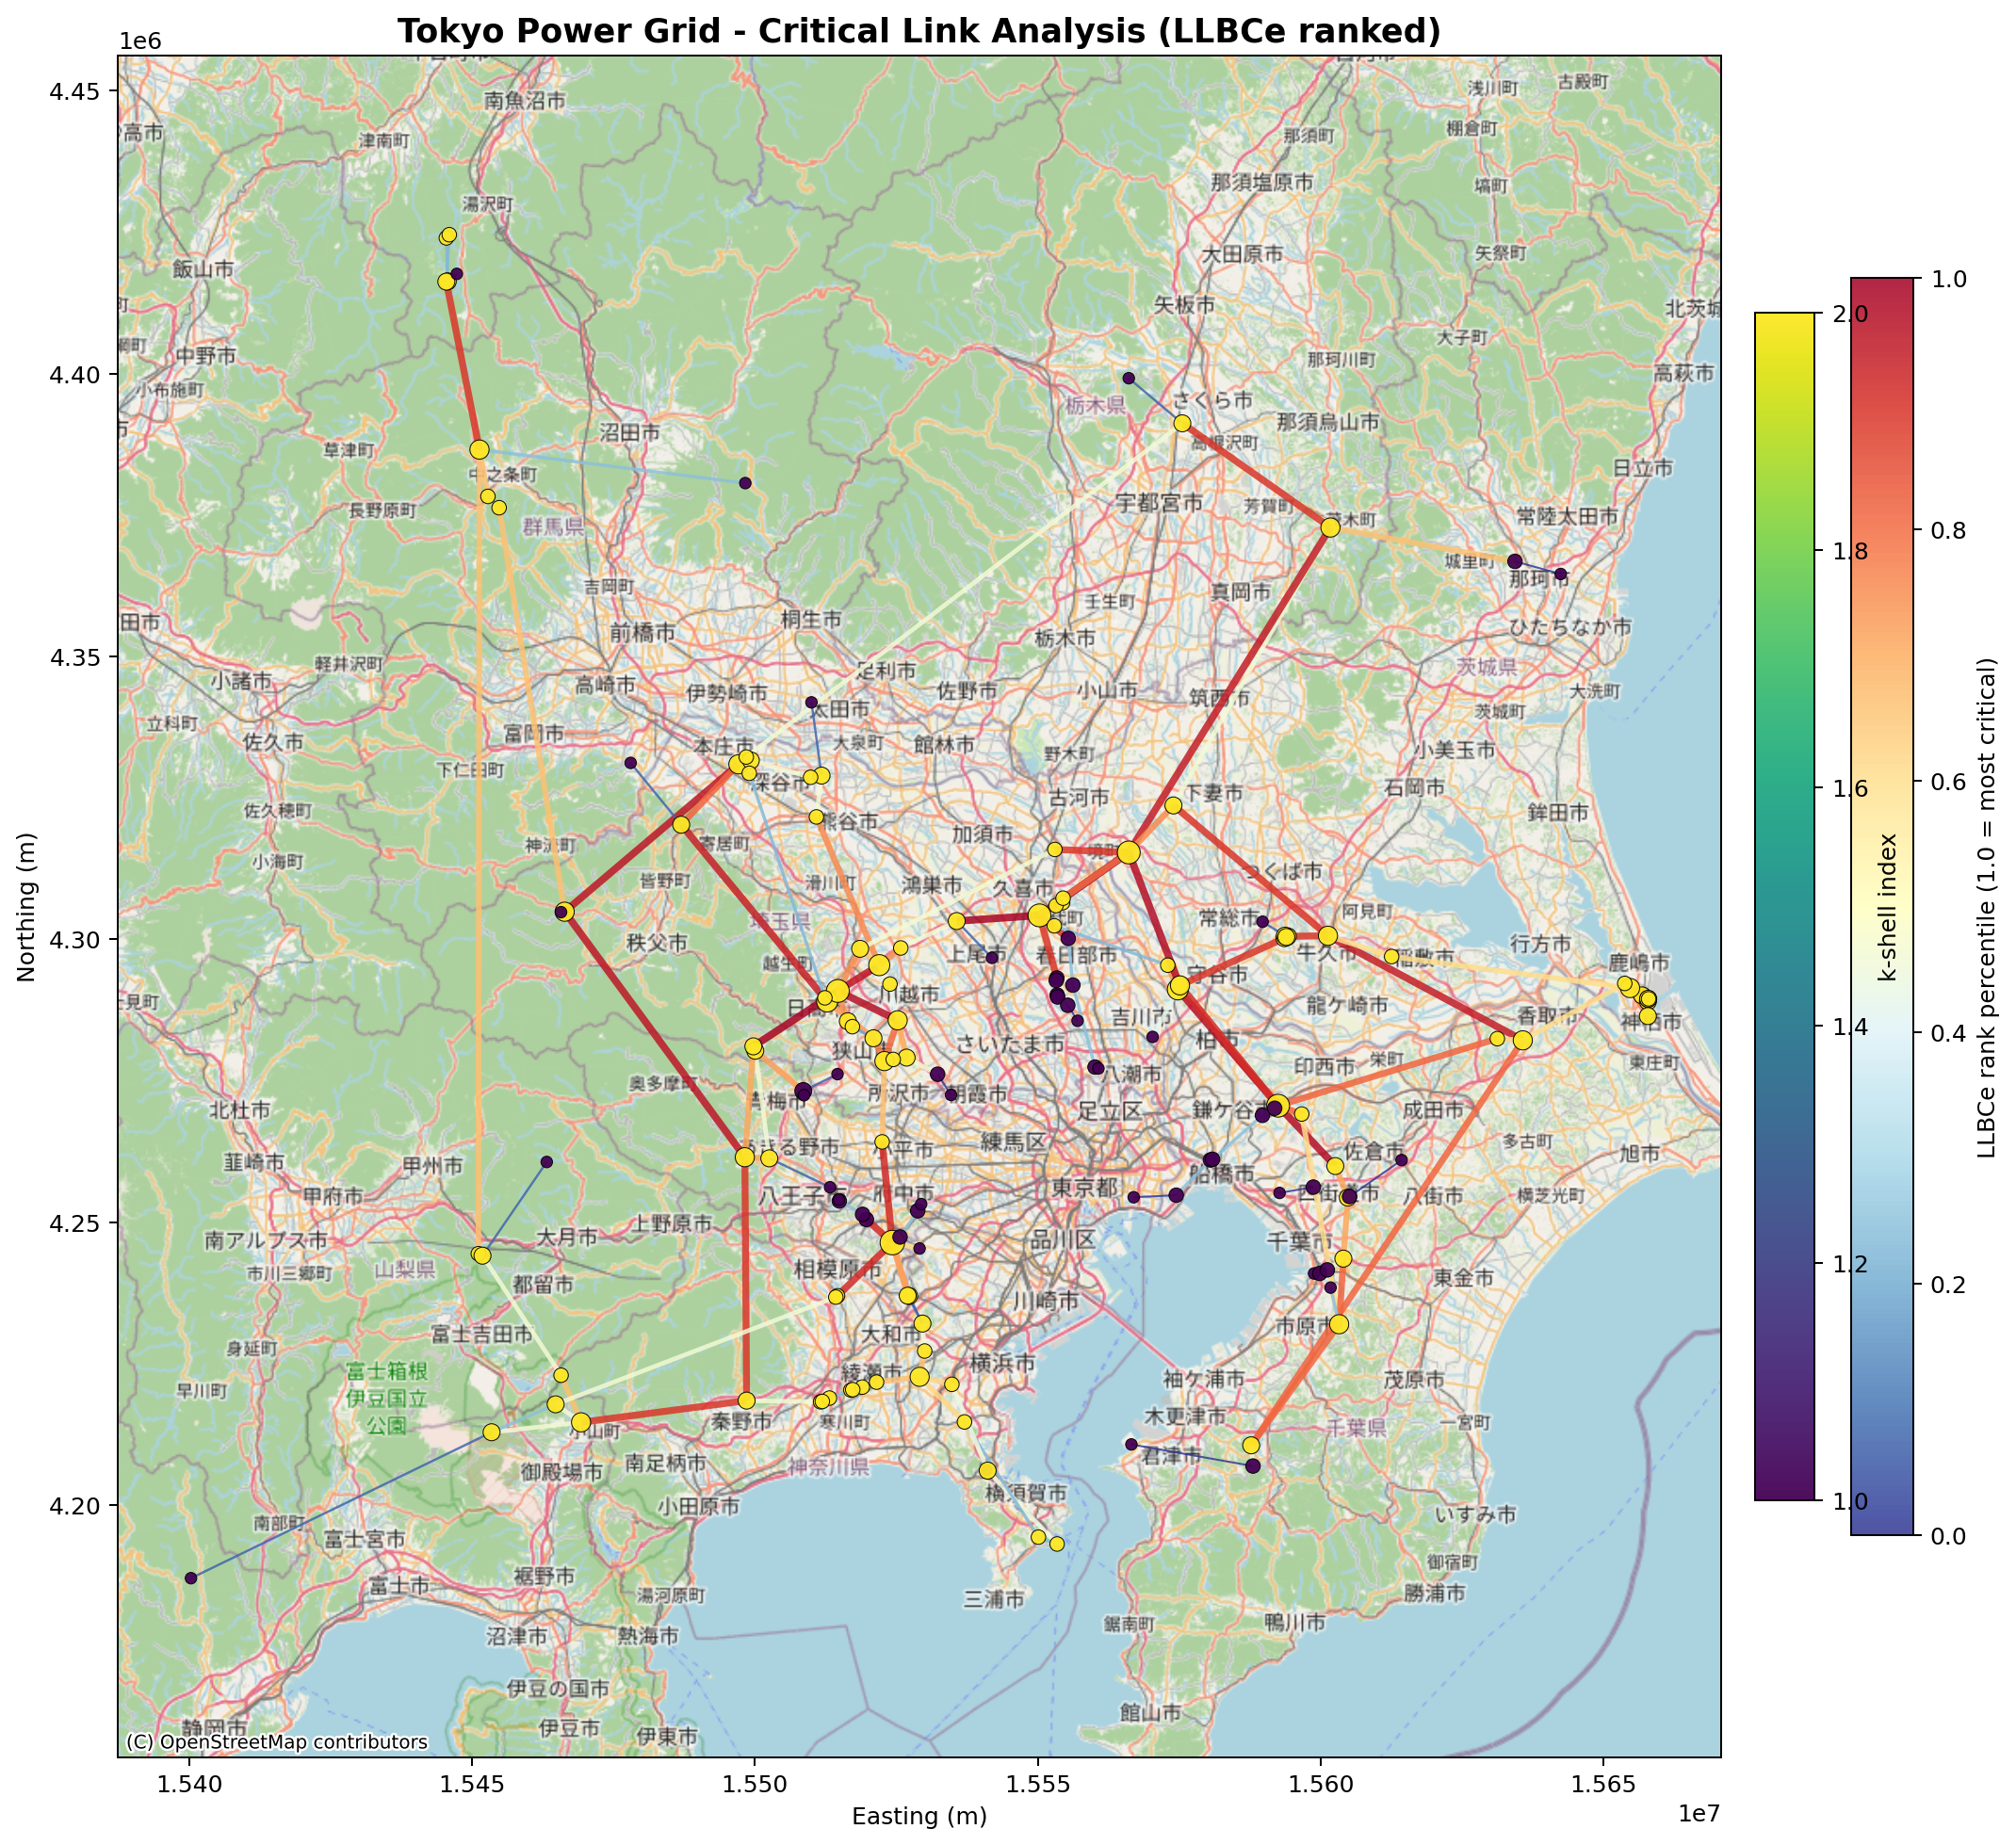
\includegraphics[width=0.92\textwidth,keepaspectratio]{../results_city/kanto_map.png}
\caption{Kanto power grid LCC over an OSM basemap. Edge colour encodes
LLBCe rank percentile (red = highest); node colour encodes $k$-shell
index. Seven trunk substations are labelled: Shin-Tokorozawa,
Shin-Tama, Shin-Keiyo, Shin-Hadano, Shin-Okabe, Shin-Haruna,
Shin-Fuji.}
\label{fig:kanto-map}
\end{figure}

\section{Discussion}
\label{sec:discussion}

\subsection{Why LLBCe wins}
The Kanto grid is a sparse ($\bar k = 2.44$), tree-like backbone with
\num{56} bridges and diameter \num{23}. In a network like this, global
betweenness on the full graph is dominated by a few edges on long
structural paths, but it is too coarse to tell them apart. LLBCe
restricts the source and target sets to the edge's first-order
neighbourhood $\Gamma(e)$, which acts as a local importance weight. It
asks: \emph{among the \num{2} to \num{12} substations within one hop of
this edge, what fraction of their pairwise shortest paths use it?} This
rescales the score to the local edge density, so a bridge in a dense
metropolitan cluster scores about the same as one in a sparse rural
area, and it stays computable on every edge in seconds even at
\num{156} nodes.

\subsection{Why CI underperforms statically}
CI was designed for node-level immunisation in scale-free networks with
heavy degree tails. The Kanto grid caps degree at \num{7}, with no
hub-and-spoke superhub, so CI's preference for high-degree nodes inside
the ball does not carry over cleanly to edge ranks. Recomputing CI
iteratively recovers much of the lost performance ($-25\,\%$ relative
AUC). The static failure is therefore about stale information, since the
CI score goes out of date right after the first removal, rather than a
flaw in the method.

\subsection{Practical implications}
The seven trunk hubs (\Cref{fig:kanto-map}) are the substations that
TEPCO lists as \SI{500}{\kilo\volt} interconnection
points~\cite{tepco2024network}. The top-ten LLBCe edges
(\Cref{tab:top-edges}) all carry a mix of \SI{275}{\kilo\volt} and
\SI{500}{\kilo\volt} feeders. Operators running $N{-}1$ contingency
analysis on this network should prioritise these corridors, and planners
weighing trunk reinforcements should treat the Shin-Koga
$\leftrightarrow$ Kita-Tokyo edge as the most exposed single-line
failure point.

\section{Threats to Validity}
\label{sec:validity}

\paragraph{OSM completeness.}
The ComplexNetTSP extraction is limited to what OSM contributors have
mapped. We checked \num{10}/\num{10} named substations against TEPCO's
illustrated facility plan, but the \num{57} unnamed line-segment vertices
suggest that some segments are over-fragmented relative to their physical
layout. TEPCO does not release authoritative data as a graph; the
closest published proxy is Toyoda et al.~\cite{toyoda2008japan}.

\paragraph{No electrical model.}
We treat the network as a topological graph with unit weights. A
production assessment would weight edges by electrical properties like
line admittance and seasonal load. The metrics here find topologically critical edges,
not necessarily electrically critical ones; the two roughly agree but
not exactly.

\paragraph{Tied-path non-determinism.}
NetworkX's \texttt{edge\_betweenness\_centrality\_subset} breaks
shortest-path ties in dict-iteration order. When many paths tie, which is
common in trunk corridors with parallel \SI{500}{\kilo\volt} and
\SI{275}{\kilo\volt} segments, LLBCe values can differ at the third or
fourth significant figure between runs. The rankings stay stable, but
reproducing the exact AUC needs the node iteration to be sorted
explicitly.

\paragraph{Frequency boundary.}
The bounding box reaches slightly west of the \SI{50}{\hertz}/\SI{60}{\hertz}
divide. In practice no Chubu (\SI{60}{\hertz}) node falls inside, but
that is luck in the data, not an explicit frequency filter. Adding a
filter on \texttt{frequency = 50} would harden the boundary.

\section{Conclusion}
\label{sec:conclusion}

The Kanto \SI{500}{\kilo\volt}/\SI{275}{\kilo\volt} backbone serves the
world's most populous metropolitan area, yet it is a sparse network whose
vulnerability comes down to a small number of bridge corridors. Across
nine edge-criticality metrics, tested under both static and iterative
dismantling, Link-Local Betweenness Centrality (LLBCe) is the most
effective ranker, with a static AUC of $0.174$ and stable iterative
performance. The top critical edges, mostly along the Shin-Koga,
Shin-Tokorozawa, and Shin-Keiyo trunks, line up with TEPCO's published
\SI{500}{\kilo\volt} interconnection map, which supports the
pure-topology approach. Future work should combine the topology with
line-admittance and capacity data to give an electrically aware
criticality score.

\section*{Reproducibility}

All code, data references, and configuration are in the
\texttt{NetworkEntropy} repository on branch \texttt{iterative-method}.
Key entry points:
\begin{itemize}
\raggedright
\item \texttt{PowerGrid\_City/\allowbreak download\_and\_filter\_tokyo.py}:
re-extracts the Kanto LCC from ComplexNetTSP CSVs.
\item \texttt{PowerGrid\_City/\allowbreak run\_city\_analysis.py}: computes the
nine metrics and writes
\texttt{results\_city/\allowbreak tokyo\_grid\_metrics.csv}.
\item \texttt{PowerGrid\_City/\allowbreak run\_iterative\_analysis.py
--method M}: iterative dismantling per metric.
\item \texttt{PowerGrid\_City/\allowbreak render\_kanto\_map.py}: folium HTML
and matplotlib PNG of \Cref{fig:kanto-map}.
\item \texttt{PowerGrid\_City/\allowbreak build\_inventory.py}: regenerates
the per-substation inventory in
\texttt{results\_city/\allowbreak tokyo\_grid\_inventory.md}.
\item \texttt{build\_comparison\_xlsx.py}: rebuilds the
cross-dataset xlsx workbook.
\end{itemize}

% --- Bibliography -----------------------------------------------------------
\begin{thebibliography}{99}
\raggedright

\bibitem{albert2004structural}
R.~Albert, I.~Albert, and G.~L. Nakarado.
\newblock Structural vulnerability of the North American power grid.
\newblock \emph{Phys.\ Rev.\ E}, 69:025103, 2004.

\bibitem{buldyrev2010catastrophic}
S.~V. Buldyrev, R.~Parshani, G.~Paul, H.~E. Stanley, and S.~Havlin.
\newblock Catastrophic cascade of failures in interdependent networks.
\newblock \emph{Nature}, 464:1025--1028, 2010.

\bibitem{tepco2024network}
Tokyo Electric Power Company.
\newblock Illustrated electricity supply: network facility plan.
\newblock \url{https://www.tepco.co.jp/en/corpinfo/illustrated/electricity-supply/network-facility-plan-e.html},
accessed April 2026.

\bibitem{braunstein2016network}
A.~Braunstein, L.~Dall'Asta, G.~Semerjian, and L.~Zdeborov\'a.
\newblock Network dismantling.
\newblock \emph{Proc.\ Natl.\ Acad.\ Sci.\ USA}, 113:12368--12373, 2016.

\bibitem{wiegmans2016gridkit}
B.~Wiegmans.
\newblock GridKit: a power-grid extract from OpenStreetMap.
\newblock \url{https://github.com/bdw/GridKit}, 2016.

\bibitem{complexnettsp2023}
ComplexNetTSP.
\newblock Power\_grids: high-voltage network extraction from OpenStreetMap.
\newblock \url{https://github.com/ComplexNetTSP/Power_grids}, 2023.

\bibitem{morone2015influence}
F.~Morone and H.~A. Makse.
\newblock Influence maximization in complex networks through optimal
percolation.
\newblock \emph{Nature}, 524:65--68, 2015.

\bibitem{kitsak2024edge}
M.~Kitsak \emph{et al.}
\newblock Edge-level Collective Influence: skin and body variants for
\(\ell\)-ball neighbourhoods.
\newblock \emph{Entropy}, 26(3):248, 2024.
\newblock \url{https://www.mdpi.com/1099-4300/26/3/248}.

\bibitem{li2024llbce}
Authors of MDPI \emph{Entropy} 26(4) 315.
\newblock Link-Local Betweenness Centrality and its mapping entropy
extension via the first-order central domain.
\newblock \emph{Entropy}, 26(4):315, 2024.
\newblock \url{https://www.mdpi.com/1099-4300/26/4/315}.

\bibitem{toyoda2008japan}
M.~Toyoda \emph{et al.}
\newblock Topological analysis of the Japanese high-voltage transmission
network.
\newblock \emph{IEEJ Trans.\ Power and Energy}, 128(3), 2008
(in Japanese).

\end{thebibliography}

\end{document}
